    \section{Derivadas Parciales}


\subsection{Objetivos del aprendizaje}
\begin{enumerate}
	\item Calcular e interpretar derivadas parciales.
	\item Aplicar derivadas parciales para estudiar Ejemplos de análisis marginal en econom\'ia.
	\item Calcular derivadas parciales de segundo orden.
	\item Usar la regla de la cadena de derivadas parciales para encontrar tasas de cambio y hacer aproximaciones incrementales. 
\end{enumerate}




\subsection{Derivadas parciales de primer orden}
La derivada parcial de $f(x,y)$ respecto de $x$ se denota por $$\partial_{x}f(x,y)\text{ \'o }f_{x}(x,y)$$ y es la funci\'on obtenida al derivar $f$ respecto de $x$ \emph{tratando a $y$ como una constante}.



\subsection{Derivadas parciales de primer orden}
De manera similar,  la derivada parcial de $f(x,y)$ respecto de $y$ se denota por $$\partial_{y}f(x,y)\text{ \'o }f_{y}(x,y)$$ y es la funci\'on obtenida al derivar $f$ respecto de $y$ \emph{tratando a $x$ como una constante}.



\subsection{Algunas propiedades y f\'ormulas}
\begin{proposicion} Sean $u(x,y),v(x,y)$ funciones de dos variables y $h(y)$ una funci\'on que no depende de $x.$
	\begin{enumerate}
		\item $\p_{x}h(y)=0;$
		\item $\p_{x}\left( h(y)u \right)=h(y)\p_{x}u;$
		\item $\p_{x}\left( u+v \right)=\p_{x}u+\p_{x}v;$
		\item $\p_{x}\left( uv \right)=u\p_{x}v+v\p_{x}u;$
		\item $\p_{x}u^{n}=nu^{n-1}\p_{x}u;$
		\item $\p_{x}e^{u}=e^{u}\p_{x}u;$
		\item $\p_{x}\ln(u)=\frac{\p_{x}u}{u}.$
	\end{enumerate}
	
\end{proposicion}




\begin{observacion}
	Las reglas siguen valiendo si: cambiamos $\p_{x}$ por $\p_y$ y $h$ no depende de $y.$
\end{observacion}




\subsection{Cálculo de derivadas parciales}

%%% Ejemplo 7.2.1


\begin{problema}
	Encuentre las derivadas parciales de $f(x,y)=x^2+2xy^2+\frac{2y}{3x}$
	
\end{problema}

El desarrollo completo del ejercicio lo puede encontrar en \href{https://youtu.be/HhCIoud7uTg}{mi Canal de YouTube.} La comprobaci\'on de la soluci\'on la puede encontrar en \href{http://sagecell.sagemath.org/?z=eJwrSyzSUK_QqVTX5OVK06jQUajUVLBVqIgz0jbSqtCqBNIaRlqVmvoaxloVICUVQDWVmrYKaXopmWlADSCxSrCYAlywEihYnJFfrpFWAWdVagIA2rkdCw==&lang=sage}{SageMathCell.}





%%% Ejemplo 7.2.2


\begin{problema}
	Encuentre las derivadas parciales de 
	$$
	f(x,y)=(x^2+x*y+y)^5.
	$$
\end{problema}
El desarrollo completo del ejercicio lo puedes encontrar en \href{https://www.youtube.com/watch?v=vT0SLF_U0mw&index=7&list=PLblwZNylw7eHCfUFZF-cc-kLIR-wzwWNi}{mi Canal de YouTube}. La comprobaci\'on se puede encontrar en \href{http://sagecell.sagemath.org/?z=eJwrSyzSUK_QqVTX5OVK06jQUajUVLBV0KiIM9Ku0KrUrtSMMwVKVABlKjVtFdL0UjLTgMpAiivBYgpwwUqgYHFGfrlGWgWcVakJAPcZGwE=&lang=sage}{http://sagecell.sagemath.org/?q=vrfhpv}


% [fragile]
% Podemos usar el siguiente c\'odigo para obtener las derivadas parciales de $f(x,y)=x^{2}+2xy^{2}+\frac{2y}{3x}:$
% \newcommand\codeHighlight[1]{\textcolor[rgb]{1,0,0}{\textbf{#1}}}
% \begin{Verbatim}
% var('x,y')
% f(x, y) = (x^2+x*y+y)^5
% fx(x,y)= f.diff(x)
% fy(x,y) = f.diff(y)
% show(fx)
% show(fy)
% \end{Verbatim}
% que se puede encontrar en \href{http://sagecell.sagemath.org/?z=eJwrSyzSUK_QqVTX5OVK06jQUajUVLBV0KiIM9Ku0KrUrtSMMwVKVABlKjVtFdL0UjLTgMpAiivBYgpwwUqgYHFGfrlGWgWcVakJAPcZGwE=&lang=sage}{http://sagecell.sagemath.org/?q=vrfhpv}
% 

% 
%  Como resultado obtenemos
% \begin{align*}
% \left( x, y \right) \ {\mapsto} \ 5 \, {\left(x^{2} + x y + y\right)}^{4} {\left(2 \, x + y\right)} \\
% \left( x, y \right) \ {\mapsto} \ 5 \, {\left(x^{2} + x y + y\right)}^{4} {\left(x + 1\right)}
% \end{align*}
% es decir,
% \begin{align*}
%  \p_{x}f(x,y)=& 5 \, {\left(x^{2} + x y + y\right)}^{4} {\left(2 \, x + y\right)} \\
%  \p_{y}f(x,y)=& 5 \, {\left(x^{2} + x y + y\right)}^{4} {\left(x + 1\right)}.
% \end{align*}
% 
% El desarrollo completo del ejercicio lo puedes encontrar en \href{https://www.youtube.com/watch?v=vT0SLF_U0mw&index=7&list=PLblwZNylw7eHCfUFZF-cc-kLIR-wzwWNi}{mi Canal de YouTube}.
% 

%%% Ejemplo 7.2.3


\begin{problema}
	Encuentre las derivadas parciales de 
	$$
	f(x,y)=xe^{-2xy}.
	$$
\end{problema}

El desarrollo completo del ejercicio lo puedes encontrar en \href{https://www.youtube.com/watch?v=2_wPr3Qnyd8&list=PLblwZNylw7eHCfUFZF-cc-kLIR-wzwWNi&index=8}{mi Canal de YouTube}. La comprobaci\'on se puede encontrar en \href{http://sagecell.sagemath.org/?z=eJwrSyzSUK_QqVTX5OVK06jQUajUVLBVqNBKrSjQ0DXSqtCqBElUAGUqNW0V0vRSMtOAykBilWAxBbggSGFxRn65RloFnFWpCQD8XBsP&lang=sage}{http://sagecell.sagemath.org/?q=onrgkx}


% [fragile]
% Podemos usar el siguiente c\'odigo para obtener las derivadas parciales de $f(x,y)=x^{2}+2xy^{2}+\frac{2y}{3x}:$
% \newcommand\codeHighlight[1]{\textcolor[rgb]{1,0,0}{\textbf{#1}}}
% \begin{Verbatim}
% var('x,y')
% f(x, y) = x*exp(-2*x*y)
% fx(x,y)= f.diff(x)
% fy(x,y) = f.diff(y)
% show(fx)
% show(fy)
% \end{Verbatim}
% que se puede encontrar en \href{http://sagecell.sagemath.org/?z=eJwrSyzSUK_QqVTX5OVK06jQUajUVLBVqNBKrSjQ0DXSqtCqBElUAGUqNW0V0vRSMtOAykBilWAxBbggSGFxRn65RloFnFWpCQD8XBsP&lang=sage}{http://sagecell.sagemath.org/?q=onrgkx}
% 
% 
% 
%  Como resultado obtenemos
% \begin{align*}
% \left( x, y \right) \ {\mapsto} \ -2 \, x y e^{\left(-2 \, x y\right)} + e^{\left(-2 \, x y\right)} \\
% \left( x, y \right) \ {\mapsto} \ -2 \, x^{2} e^{\left(-2 \, x y\right)}
% \end{align*}
% es decir,
% \begin{align*}
%  \p_{x}f(x,y)&=   -2 \, x y e^{\left(-2 \, x y\right)} + e^{\left(-2 \, x y\right)} \\
%  \p_{y}f(x,y)&=  -2 \, x^{2} e^{\left(-2 \, x y\right)}.
% \end{align*}
% 
% El desarrollo completo del ejercicio lo puedes encontrar en \href{https://www.youtube.com/watch?v=2_wPr3Qnyd8&list=PLblwZNylw7eHCfUFZF-cc-kLIR-wzwWNi&index=8}{mi Canal de YouTube}.
% 
% 


\begin{problema}
	Evalue las derivadas parciales $\p_{x}f(x,y)$ y $\p_{y}f(x,y)$ en el punto $(x_{0},y_{0})$ dado:
	\begin{enumerate}
		\item $f(x,y)=x^{3}y-2(x+y), \ x_{0}=1, y_{0}=0;$
		\item $f(x,y)=x+\dfrac{x}{y-3x}, \ x_{0}=1, y_{0}=1;$
		\item $f(x,y)=(x-2y)^2+(y-3x)^2+5, \ x_{0}=0, y_{0}=-1;$
		\item $f(x,y)=xy\ln{\left( \dfrac{y}{x} \right)}+\ln{\left( 2x-3y \right)^{2}}, \ x_{0}=1, y_{0}=1;$
	\end{enumerate}
	
\end{problema}

Puede verificar sus resultados con este \href{http://sagecell.sagemath.org/?z=eJxtkE1uwyAQhfeWfIcRWYSktOrP2steI9UUg4REiYUhmjlXj5CLdey2kVtbLHiC9958sOudjZjx4zxCxBEumAO-RzcCQ6puLBnB12TD9TO1DRmGbvLovcj9oW28FnGQQzq9HBnu4fmo6Y7lZsiuFH4bckhFq5tPGfjWYmmbncVoa7yNHzDbgDJemmm2df6hD14i60padtJvqec_uQ0UXuZ4AeMuGOvM4hJE2Yaaimwh9cFifxYqkthT20zf8Pi_-HWOZzcVUCflZEABT2qDgrQyZJQsNmr1ihXyhvkH_QtIfoik&lang=sage}{este script.}


\subsection{Clasificaci\'on de Puntos Cr\'iticos}


\begin{definicion}[Extremos relativos]
	Diremos la función f(x,y)
	tiene un \emph{máximo relativo} en $(x_{0},y_{0})$ si $$f\left( x_{0},y_{0} \right) \geq f(x,y)$$ 
	para todo $(x,y)$ suficientemente cercano a $(x_{0},y_{0}).$ 
	
	De manera similar, diremos la función f(x,y)
	tiene un \emph{m\'inimo relativo} en $(x_{0},y_{0})$ si $$f\left( x_{0},y_{0} \right) \leq f(x,y)$$ 
	para todo $(x,y)$ suficientemente cercano a $(x_{0},y_{0}).$ 
	
\end{definicion}




Los \emph{extremos relativos} no siempre son \emph{extremos absolutos}...
\begin{figure}
	\centering
	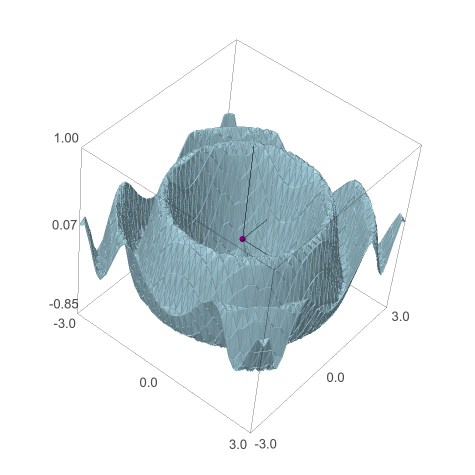
\includegraphics[height=5cm]{./cvv/cvv04.png}
	% cvv04.png: 0x0 pixel, 300dpi, 0.00x0.00 cm, bb=
	\caption{Máximo Relativo}
	\label{fig:04}
\end{figure}

Est imagen la puede genera con el siguiente c\'odigo: \href{http://sagecell.sagemath.org/?z=eJw9jkFuwyAQRfeWfIeRNwGbUFOrm0rcIVK6r3A8DqjYUMCt3dOXxE1nFqP3pdH7A44wkpVt9LUsIE_AtIQZyFHQelJJ82hmstVbs9YrfdqTz5BIxuYW87ZtBS2LsjiBBG9d6gYyMnLsWEcfB9SgfDJfKN_CggwuzrogK2uuOvV2wQoYTGp973EeJBc7DOiTluIlE0Z9_8yeMbgJoroiv7n4Lvw7YCbvQgK1YiyLc-5zguZORDykh96qy8eBNuCdmRMhLcubK0bzg1I8_5fzS_AWq6w886jdN6G_zYpbDw==&lang=sage}{http://sagecell.sagemath.org/?q=wdxppk}



Sin embargo, para puntos suficientemente cercano, un \emph{extremo relativo} s\'i lo es.
\begin{figure}
	\centering
	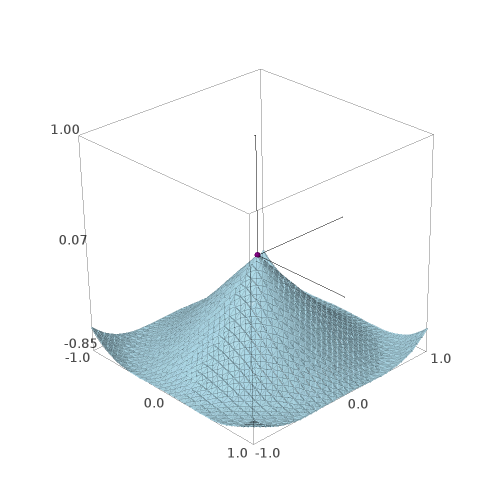
\includegraphics[height=5cm,keepaspectratio=true]{./cvv/cvv05.png}
	% cvv05.png: 0x0 pixel, 300dpi, 0.00x0.00 cm, bb=
	\label{fig:05}
\end{figure}

Esta imagen la puede generar con el siguiente c\'odigo:
\href{http://sagecell.sagemath.org/?z=eJw9jsFuwyAQRO-W_A8rXwI2pUZVe6jEP0RK7xWO1wEVGwq4xf36krjp7mE0I43ejDjBRDLb6GtdQbmAaQ0LkAdB21klzaNZyNZuXW4zfdyTz5BIsd015n3fC1pXdXUECd669DSSiZU-E_QuoEblk_lC-RZWZHB21gXZWHPRabArNsBgVvl9wGWUXOxmRJ-0FM_FYdS3ZuFMwc0Q1QX5lcV34J-Amb0LCVTGWFensucI3c0RcYceBqvOHwfagXdmSYT0rHyZGM0PSvHyP86vwVtsCvLEo3bfhP4Cx45bCw==&lang=sage}{http://sagecell.sagemath.org/?q=butszu}



De hecho, el mapa topográfico de la regi\'on, nos indica que existen punto a una mayor altura que el \emph{máximo relativo.}

\begin{figure}
	\centering
	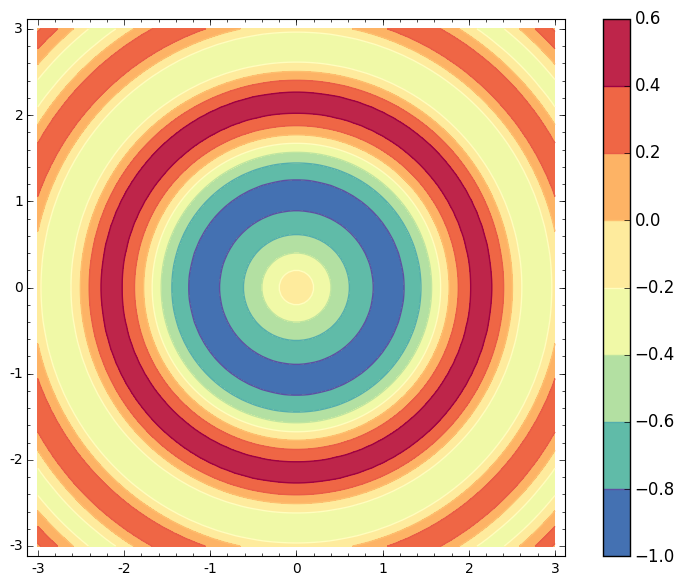
\includegraphics[height=5cm,keepaspectratio=true]{./cvv/cvv06.png}
	% cvv06.png: 0x0 pixel, 300dpi, 0.00x0.00 cm, bb=
	\caption{Mapa topográfico con alturas}
	\label{fig:06}
\end{figure}

Puede generar este mapa topográfico con el siguiente c\'odigo \href{http://sagecell.sagemath.org/?z=eJxFjMEKwjAQRO-C_5BbNmmqKT3nK-q9xFBBiN24TSX7927x4Gkej5lpjlVQn0igm2NtzqcHCJgA_WDs9lyBLXfNNnPd3lRBqDvMxXs_SDvhWnGnuWSs8Js6JaH60anxYP5zesUS9FSWVCnmmbQozEj3SOFG-yJ_X4w9KWI=&lang=sage}{http://sagecell.sagemath.org/?q=zyutmy}



\begin{definicion}[Puntos cr\'iticos]
	Un punto $(x_{0},y_{0})$ es un \emph{punto cr\'itico} de $f(x,y)$ si
	$$
	\p_{x}f(x_{0},y_{0})=0, \ \p_{y}f(x_{0},y_{0})=0.
	$$
\end{definicion}

Todos los extremos relativos son puntos cr\'iticos...



Pero no todos los puntos cr\'iticos son extremos relativos.

\begin{figure}
	\centering
	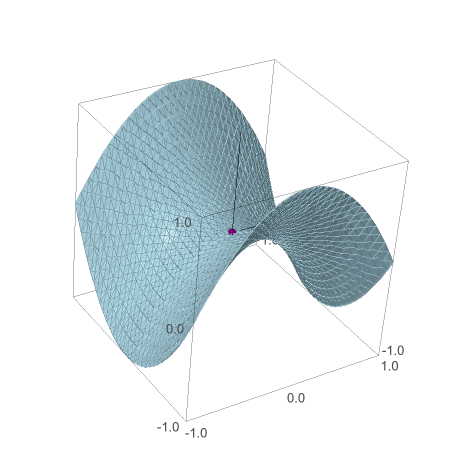
\includegraphics[height=5cm,keepaspectratio=true]{./cvv/cvv07.png}
	% cvv07.png: 0x0 pixel, 300dpi, 0.00x0.00 cm, bb=
	\caption{Punto de silla}
	\label{fig:07}
\end{figure}

\href{http://sagecell.sagemath.org/?z=eJw9jsGOwiAURfck_MNLN0KkzeDEWUzCP5jUtYbKqyVDCwE6Vr9e1HHeW9ycxc25Bnvo2SKu_JsSKBcxz3GC62FTL4cNJZTsQEFwPn8a1gtWSyH5O0AbHbL9RbWPMwo4eeejqpw9D7lzM1YgYNTLscPJqEa-wGDIg5LbQpiGZ5NT0kc_QtJnbB6u5iX8C7Bj8DGDXjBR0pY9O1g_icm3dNU5ffpZ8TUEb6fM2IcoXyYme0Mlv_7HhTkGh1VRtk0a_IXxO58zTv8=&lang=sage}{http://sagecell.sagemath.org/?q=kmfhcx}



Diremos que un punto cr\'itico que no es extremo local es un punto de silla. 




\begin{figure}
	\centering
	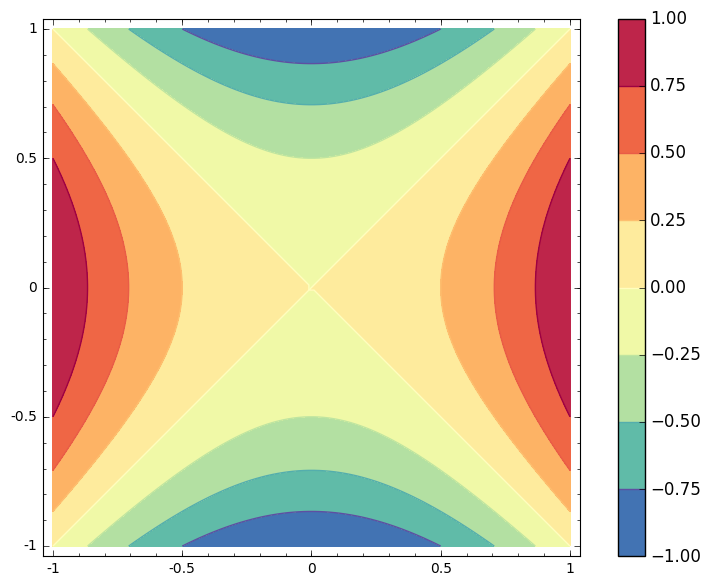
\includegraphics[height=5cm,keepaspectratio=true]{./cvv/cvv08.png}
	% cvv08.png: 0x0 pixel, 300dpi, 0.00x0.00 cm, bb=
	\caption{Mapa topografico de $f(x,y)=x^2-y^2$}
	\label{fig:08}
\end{figure}

\href{http://sagecell.sagemath.org/?z=eJyr0KlUsFUoSyzSUK_QqVTX5OVK0wAyNG0r4ox0K-OMeLmS8_NK8kuL4gty8ks0IJI6CkBKQddQR8EQxK5EsJNzEwts1YMLUpNLihJz4ovUgUL5OflFSYlFtiFFpamaAAuqIOc=&lang=sage}{http://sagecell.sagemath.org/?q=mjknwh}

\begin{observacion}
	$(0,0)$ es punto de silla de $f(x,y)=x^2-y^2.$
\end{observacion}




\begin{definicion}[Segundas derivadas] Las derivadas parciales de segundo orden de $f(x,y)$ son
	\begin{itemize}
		\item $\p_{xx}f(x,y)=\p_{x}\left( \p_{x} f(x,y) \right)=f_{xx}(x,y)$
		\item $\p_{xy}f(x,y)=\p_{x}\left( \p_{y} f(x,y) \right)=f_{yx}(x,y)$
		\item $\p_{yx}f(x,y)=\p_{y}\left( \p_{x} f(x,y) \right)=f_{xy}(x,y)$
		\item $\p_{yy}f(x,y)=\p_{y}\left( \p_{y} f(x,y) \right)=f_{yy}(x,y)$
	\end{itemize}
	
\end{definicion}



\subsection{Hessiano de una funci\'on}
\[
	\label{hess}  
	\operatorname{Hess}f(x,y)=
	\begin{pmatrix}\p_{xx}f(x,y) &\p_{yx}f(x,y) \cr \p_{xy}f(x,y) & \p_{yy}f(x,y) \end{pmatrix}
\]





El determinante Hessiano de $f(x,y)$ se define como
$$
D(x,y)=\p_{xx}f(x,y)\p_{yy}f(x,y)-\p_{xy}f(x,y)\p_{yx}f(x,y).
$$



\begin{observacion}
	Si las derivadas parciales mixtas $\p_{xy}f(x,y), \ \p_{yx}f(x,y)$ existen y son continuas, entonces
	$$
	\p_{xy}f(x,y)=\p_{yx}f(x,y),
	$$
	de manera que 
	$$
	D(x,y)=\p_{xx}f(x,y)\p_{yy}f(x,y)-\left( \p_{xy}f(x,y) \right)^{2}.
	$$
\end{observacion}




\begin{teorema}[Clasificaci\'on de puntos cr\'iticos]
	Supongamos que todas las derivas de primer y segundo orden de $f(x,y)$ existe y que $(x_{0},y_{0})$ es un punto cr\'itico de $f(x,y).$ Entonces
	\begin{itemize}
		\item Si $D(x_{0},y_{0}) < 0,$ entonces $(x_{0},y_{0})$ es un \emph{punto de silla}.
		\item Si $D(x_{0},y_{0}) > 0$ y $\p_{xx}f(x_{0},y_{0})>0,$ entonces $(x_{0},y_{0})$ es un \emph{m\'inimo relativo}.
		\item Si $D(x_{0},y_{0}) > 0$ y $\p_{xx}f(x_{0},y_{0})<0,$ entonces $(x_{0},y_{0})$ es un \emph{máximo relativo}.
	\end{itemize}
	
\end{teorema}

\begin{observacion}
	Si $D(x_{0},y_{0}) = 0,$ la informaci\'on no es concluyente.
\end{observacion}




\begin{problema}
	Clasifique los puntos cr\'iticos de $f(x,y)=x^{2}+y^{2}.$
\end{problema}

Puede ver el desarrollo completo del ejercicio en \href{https://www.youtube.com/watch?v=9Vz-qouiRPw}{https://youtu.be/9Vz-qouiRPw}. 

Para encontrar los puntos cr\'iticos, puede \href{http://sagecell.sagemath.org/?z=eJyNkcFqwzAMQO-B_IOghyYsjNDryGndD-w6VlBcBQSO49lxiD9nH7DTPiE_NsVtSo47GGRLT0_IhzN1bLgfPGj0MKFjbDX5PJOwOM5VPJYveXbYl0EXjOLl18j7mwHyI4FFP8CVWgKFfcvo9nVgh3T_CiSHySHQhDqgy7OumCuIJTQwX05PEC8n6fqKWgWNd51Fpxg1OPKW1Lh6YBZyFjSWDXTPV-6kT_kvMgoZEwkPNK7oO_lBT7StglRAxYMhL5QGG4zwyi0_I6sBNnldwb1bU9_WkbRmRC2BJ-DeOu7ZLd9rRrMfcZ1CVOHWvYJkUOyqNZE8_iGSj0hTFR-bca9s6s8K0v7yLM_-ALxgmeU=&lang=sage}{este script.}

Para evaluarlos en $D(x,y)$ y $\p_{xx}f(x,y)$ puede utilizar \href{http://sagecell.sagemath.org/?z=eJyNkUtqw0AMhvcG30GQRWwaQsm2eNUU0ksElLGcDow17jzCuHfqqkfIxarYMXW7SLMYNI9_Pkm_FltqNOvWejDo4YRO48GQzzPZFsu06pflU54t5jJoIit9_mK5f2EgHwg69BZqOhAobA8a3VwHnR3O75FkaXIIdEIT0eVZU6QV9CVUkPabB-j3m4GqLAeH13wtBqc_YEfea2TMs13VrN_GU1H-0fsodQRyrWaUCrfC78tqN4S1vAwfntGoaCa-p2PkGqUJpzQacOQ7UuHSECQpMaURAs261o1UXE5RUK98FP2EUta6mhiFli7fOYo9zkIXWXjKnT-DVhZmBqTq8Ralv4_Sj5S2c7odxkTiOnJAIzgyMlgjM6hl92OOjO1qqb3I5e03P8-ExqEYLSzv4v9r581Mk9OS6xvaZ-WA&lang=sage}{este script.}



\begin{problema}
	Clasifique los puntos cr\'iticos de $f(x,y)=12x-x^3-4y^{2}.$
\end{problema}

Puede ver el desarrollo completo del ejercicio en \href{https://www.youtube.com/watch?v=oY3DjTSqado}{https://youtu.be/oY3DjTSqado}.

Para encontrar los puntos cr\'iticos puede usar \href{http://sagecell.sagemath.org/?z=eJyNkUFqwzAQRfcG32Egi9jBKW6aXfGq7QW6LQ2MlTEMyLIrWcY6Tg_QVY_gi3WsxCHLLgSSZt5_YrR5pYYNt50DjQ5GtIy1Jpcmss22UxG2-XOabO7boPFG8fxr5P7NALmBoEfXwZlqAoVtzWjv-6Dv4vnLkywmi0Ajao82TZpsKiDkUMHjYTftp9PT_rgLp4Nkv6BWXuNV2qNVjBosuZ7UsNhgEn6SgJBX0DycuZG0_F9kEDJEEm5oWNB3cp0eaR0IKY-KO0NOKA29N8IrO_8MrDpY5WUB17SqvAwlas2AWjaOgNvecst2_l4qmt2AyytE5S_pBUSDYlsshehxN5F8R3xV9rEa75VV-VlAnGKapMkfr0ibWA==&lang=sage}{este script.}

Para evaluarlos en $D(x,y)$ y $\p_{xx}f(x,y)$ puede utilizar \href{http://sagecell.sagemath.org/?z=eJyNkU1uwjAQhfeRcoeRWBAjQC3trsqqVKKXQBqcCbXk2Kl_kNM7ddUjcLFOAlFpF5SFZY89883zm8maamVUYz1o9HBAp3CnyecZH4tpmndT8ZRnk8s0qKOR6vhl-P7FAPlA0KK3UNGOQGKzU-gu86C1Q_weiZcih0AH1BFdntVFmkMnoIT71Swt0vZh8TjrtquBLa0JDs9dGwxOfcCGvFdoMM82Zb18O0WF-JPvI6sJ5BplkHWuuUsnys2wLfllKHhGLaMe-Z720VTIX3FSoQZHviUZ-m9BYqEpnSBQLytVs24x7nnGsFez54oRJq11FRlkXuoBJrJNzkIbDROlO34GJS1cGJHKxeoaprsN05V3PaVpnWqGeRHbjyagZhxpnrDmYVR8-vGH53d21fbp_Pabn2dMM6E4uShu4v_r6NVOo9niG9bV5yI=&lang=sage}{este script.}



\begin{problema}
	Clasifique los puntos cr\'iticos de $f(x,y)=x^3-y^3+6xy.$
	
\end{problema}

Puede ver el desarrollo completo del ejercicio en \href{hhttps://www.youtube.com/watch?v=oCk2O9SpJG4}{https://youtu.be/oCk2O9SpJG4}.

Para encontrar los puntos cr\'iticos puede usar \href{http://sagecell.sagemath.org/?z=eJyNkb1qwzAUhXeD3-FChsSpWgKBLsVT26Fr19LAjXJdLsiSK1nBepw-QKduXf1ivVZ-8NjBIEv6zjk6d_FEDVtuXQCDAY7oGfeGQlnIcrUcVFpWD2WxmF-DJlrN44-V_WcLFHqCDoODA-0JNLZ7Rj-_B53L_5-R5GPyCHREE9GXRbMaFKQKahh229u0297cr4d1EulHNDoaPHt26DWjAU-hI91PZjAIPgifqhqauwM3Ilb9ixT9JmUSrmia0FcKzhzp0gfpiJqdpSCUgS5a4bUfv3vWDi7mGwVntXpz6iTb2h6NLAIBt53nlv34NZ0YDj1OKcQqntQVZAfNXk0H2SdcjcKsaC1FK3At93kaKJ2aKenBWQFRHkuaQLLa8bcl78QbP9jKXB28lEV-3ertknwevd68K8jDKIuy-AMe8LWb&lang=sage}{este script.}

Para evaluarlos en $D(x,y)$ y $\p_{xx}f(x,y)$ puede usar \href{http://sagecell.sagemath.org/?z=eJyNkU1uwjAQhfeRcoeRWBBTYFGkbqqsSiV6CaTBmVBLjp36B9m9U1c9AhfrEIhKu6BdWPbYM9-M35usqVVGddaDRg8HdAp3mnxZ8LGapnmeiseymFynQRuNVMdPw_fPBsgHgh69hYZ2BBK7nUJ3nQe9HeK3SLwUOQQ6oI7oyqKt0hyygBrSdrXI29XdwyzN8oCW1gSHl6YdBqfeYUPeKzRYFpu6Xb6eo0r8yveRhwnkOmWQx1xzkyzqzbAt-WUoeEItox75nvbRNMg_cVKhBke-JxlOv4LEc6Z0hkC7bFTLY4txLwuGvZg9V4wwaa1ryCDz0glgIqvkLPTRMFG640dQ0sKVDqm-v0XJ_6PkejFgut6pbrCLWH00ATXzSLPBmr1o-PStD9t3UdWe0vntZ4OyYJoJ1VlF8S_-n4re7DSKLb4A5KvnOw==&lang=sage}{este script.}





\begin{problema}
	Clasifique los puntos cr\'iticos de cada una de las siguientes funciones:
	\begin{enumerate}
		\item $f(x,y)=5-x^2-y^2$
		\item $f(x,y)=\frac{16}{x}+\frac{6}{y}+x^2-3y^2$
		\item $f(x,y)=x^3+y^2-6xy+9x+5y+2$
		\item $f(x,y)=(x^2+2y^{2})e^{1-x^2-y^2}$
	\end{enumerate}
	
\end{problema}

Puede verificar sus resultados, utilizando este \href{http://sagecell.sagemath.org/?z=eJyVVMGK2zAQvRv8D4NyWBu8ISz00l33slnIpaW0x9JdxrJMBYoUJDvYn9MP2FM_IT_WkWIr3iQLbUISWXrz3szoTRa14Aotbo0DhQ72aCVWSrg06YuhpMfshhY3-X2apMmiFo3U0oN1J1xrEZpOc3n4o8NhJYDjtpJoiQyO4HBKa78zgf0j8k7Y2gAq2FlDkltMkybrCxhyKOHDbf98dzs833ndnRVtO7zsrNRtxjwoYFgBx3VO6hwV71QsZIeWSwyFNH0AldAsa9lQRH7B2M8p-4mzGabtMXK4jBzmkUPM5rtRHZdGj_mA4B1OpVPBnW4NcHt4bSU3npPIgD0FkNHCXUGxM-kxzQIYia_YeWZjLrNjJV1bOqP2IvsxtaRcxaxp_bOA0P6Y0FSFcKTeGDumJDV4so9pAvR6IxsAvgGPp-ugUn4J5yRqAwO4DmrpuJVbqVG3Ik02ZbMcAdlJezOGnNcdDmDugc3U9fWxkOPzshbtjG4914R3ydcz3nX0QT-2KxrofSO9dVK00kLsUXVHN9AntMnFu3X3x7kR4ZCQxpIH-hLpNsrKe5kcFAgsAWuEjlpJM0QjaMjgWK7SpPJfsdxHmgHZSB5NdyHJLgfr6dxzcJKlfLBkBRYMKvqtLkpfZ0i7U-f8-tqYnTC-OSMqTWQzxjysrrmKZUGZ3lXBcgpmlM7XkCpV5qRS6B0uVOT5NPHQzqQU9_6N__Ph1f_VwTehsJV74xV8ZFCZOB_-l_N3f84plBNXi_5iwPl7E1QjmVlY717L8r-wl8z7&lang=sage}{este script.}


% 
%  \begin{problema}
%   El departamento de carreteras planea construir un área de merenderos para automovilistas a lo largo de una carretera principal. Debe ser rectangular con un área de 5000 yardas cuadradas y debe estar cercado en los tres lados no adyacente a la carretera. ¿Cuál es la cantidad m\'inima de cercado necesaria para completar el trabajo?
%  \end{problema}
% 
% 
% 
% 
%  \begin{figure}
%  \centering
%  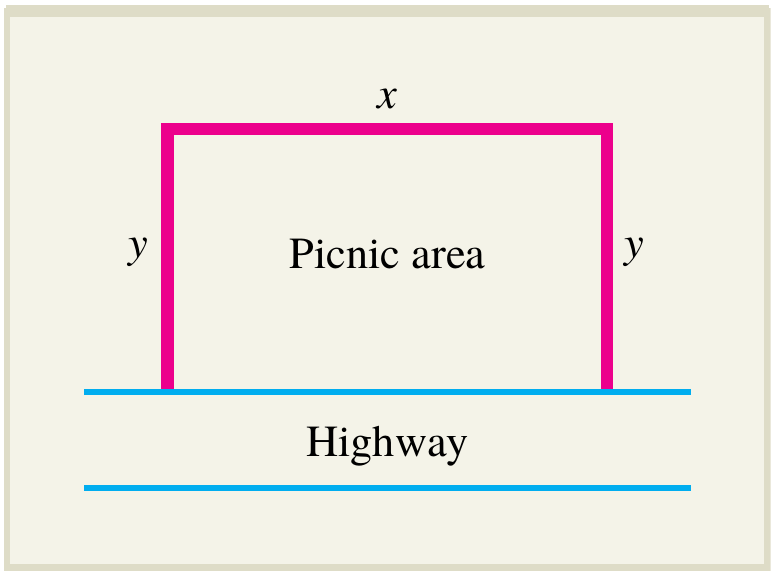
\includegraphics[height=3cm,keepaspectratio=true]{./cvv/cvv09.png}
%  % cvv09.png: 0x0 pixel, 300dpi, 0.00x0.00 cm, bb=
%  \caption{\'Area rectangular de merenderos}
%  \label{fig:09}
% \end{figure}
% 
% El problema es \emph{minimizar} $f(x,y)=x+2y$ restringida por $$g(x,y)=5000.$$
% 
% 
% 
% 
% 

